\documentclass[12pt]{article}

\usepackage{answers}
\usepackage{setspace}
\usepackage{graphicx}
\usepackage{enumitem}
\usepackage{multicol}
\usepackage{mathrsfs}
\usepackage[margin=1in]{geometry} 
\usepackage{amsmath,amsthm,amssymb}
\usepackage{pgfplots}
\usepackage{listings}
\pgfplotsset{compat=1.15}
\usepgfplotslibrary{fillbetween}
 
\newcommand{\N}{\mathbb{N}}
\newcommand{\Z}{\mathbb{Z}}
\newcommand{\C}{\mathbb{C}}
\newcommand{\R}{\mathbb{R}}

\DeclareMathOperator{\sech}{sech}
\DeclareMathOperator{\csch}{csch}
 
\newenvironment{theorem}[2][Theorem]{\begin{trivlist}
\item[\hskip \labelsep {\bfseries #1}\hskip \labelsep {\bfseries #2.}]}{\end{trivlist}}
\newenvironment{definition}[2][Definition]{\begin{trivlist}
\item[\hskip \labelsep {\bfseries #1}\hskip \labelsep {\bfseries #2.}]}{\end{trivlist}}
\newenvironment{proposition}[2][Proposition]{\begin{trivlist}
\item[\hskip \labelsep {\bfseries #1}\hskip \labelsep {\bfseries #2.}]}{\end{trivlist}}
\newenvironment{lemma}[2][Lemma]{\begin{trivlist}
\item[\hskip \labelsep {\bfseries #1}\hskip \labelsep {\bfseries #2.}]}{\end{trivlist}}
\newenvironment{exercise}[2][Exercise]{\begin{trivlist}
\item[\hskip \labelsep {\bfseries #1}\hskip \labelsep {\bfseries #2.}]}{\end{trivlist}}
\newenvironment{solution}[2][Solution]{\begin{trivlist}
\item[\hskip \labelsep {\bfseries #1}]}{\end{trivlist}}
\newenvironment{problem}[2][Problem]{\begin{trivlist}
\item[\hskip \labelsep {\bfseries #1}\hskip \labelsep {\bfseries #2.}]}{\end{trivlist}}
\newenvironment{question}[2][Question]{\begin{trivlist}
\item[\hskip \labelsep {\bfseries #1}\hskip \labelsep {\bfseries #2.}]}{\end{trivlist}}
\newenvironment{corollary}[2][Corollary]{\begin{trivlist}
\item[\hskip \labelsep {\bfseries #1}\hskip \labelsep {\bfseries #2.}]}{\end{trivlist}}
 
\begin{document}
 
% --------------------------------------------------------------
%                         Start here
% --------------------------------------------------------------
 
\title{In-Class Assignment - CSP}%replace with the appropriate homework number
\author{Basil R. Yap\\ %replace with your name
50.021 Artificial Intelligence - Term 8} %if necessary, replace with your course title
\date{July 26, 2018}
\maketitle
%Below is an example of the problem environment

% Question 1
\begin{figure}[h!]
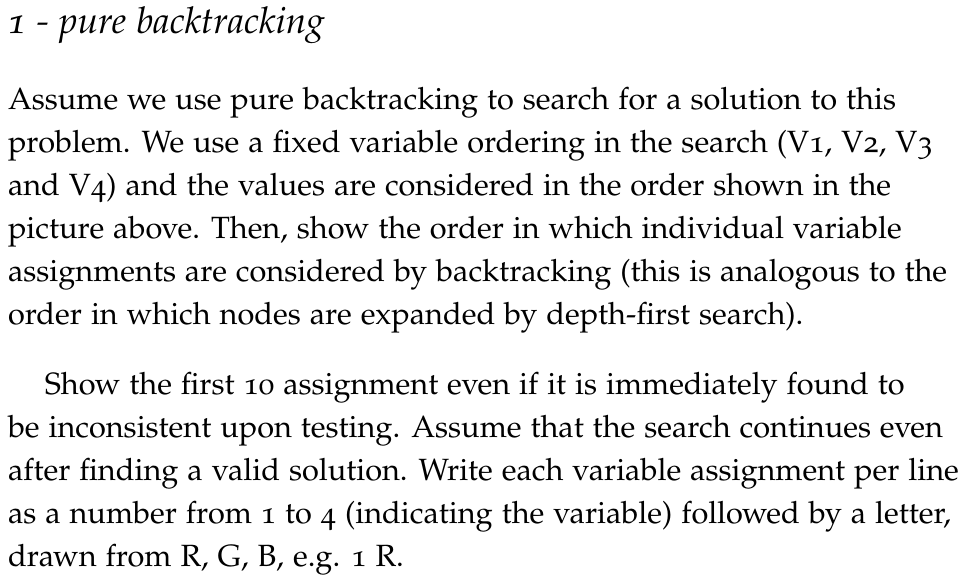
\includegraphics[width=\linewidth]{./assets/201807261942.png}
\end{figure}

\begin{solution}{}~\\
The sequence of the pure backtracking search are as follows:\begin{enumerate}
\item 1R
\item 1R2B
\item 1R2B3B [INVALID]
\item 1R2B3G
\item 1R2B3G4B [INVALID]
\item 1R2G
\item 1R2G3B
\item 1R2G3B4B [INVALID]
\item 1R2G3G
\item 1R2G3G4B [STOP / SOLVED]
\end{enumerate}
\end{solution}

% Question 2
\begin{figure}[h!]
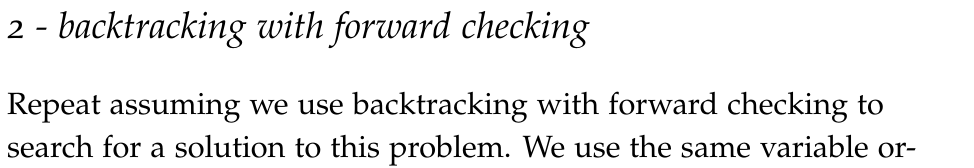
\includegraphics[width=\linewidth]{./assets/201807261943.png}
\end{figure}
\begin{figure}[h!]
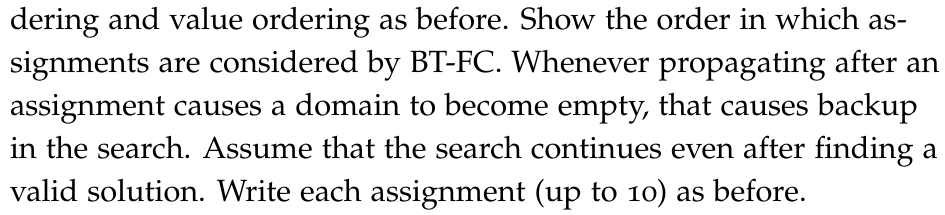
\includegraphics[width=\linewidth]{./assets/201807261944.png}
\end{figure}

\begin{solution}{}~\\
The sequence of the pure backtracking search are as follows:\begin{enumerate}
\item 1R
\item 1R2B [INVALID]
\item 1R2G 
\item 1R2G3B [INVALID]
\item 1R2G3G 
\item 1R2G3G4B [STOP / SOLVED]
\item 1B
\item 1B2G
\item 1B2G3G
\item 1B2G3G4B [STOP / SOLVED]
\end{enumerate}
\end{solution}

% Question 3
\begin{figure}[h!]
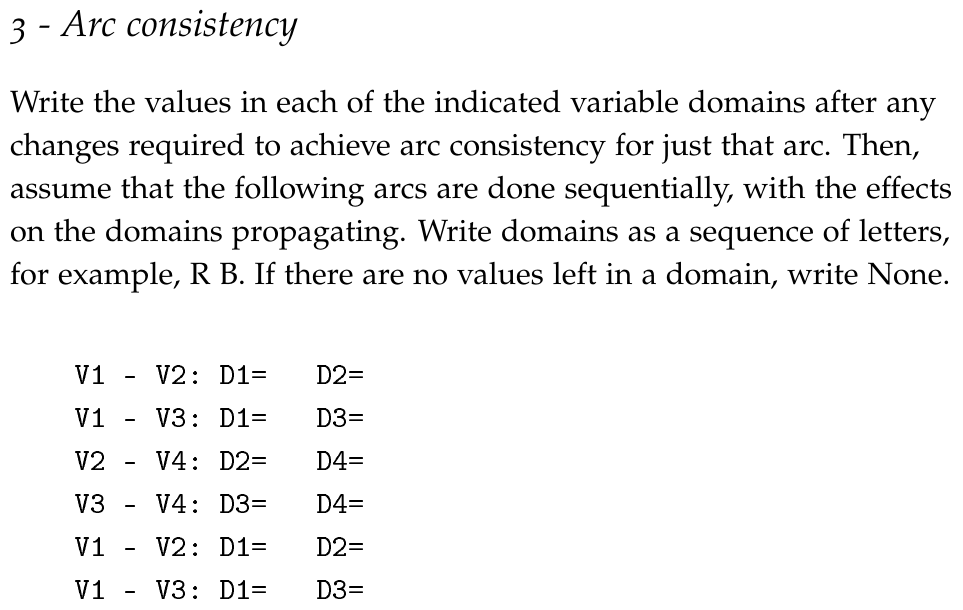
\includegraphics[width=\linewidth]{./assets/201807261945.png}
\end{figure}

\begin{solution}{}~
\begin{center}
\begin{tabular}{| c | l | l |}
\hline
V1-V2 & D1 = RGB & D2 = GB\\
V1-V3 & D1 = RGB & D3 = GB\\
V2-V4 & D2 = G & D4 = B\\
V3-V4 & D3 = G & D4 = B\\
V1-V2 & D1 = RB & D2 = G\\
V1-V3 & D1 = RB & D3 = G\\
\hline
\end{tabular}
\end{center}
\end{solution}
\pagebreak
% Question 4
\begin{figure}[h!]
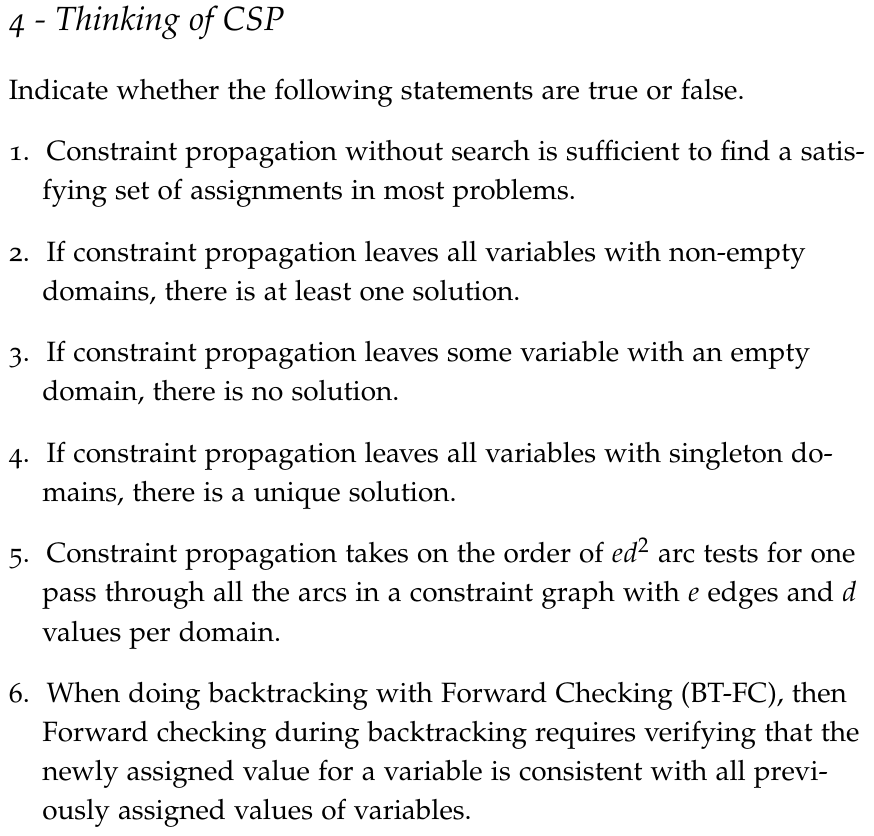
\includegraphics[width=\linewidth]{./assets/201807261946.png}
\end{figure}
\begin{figure}[h!]
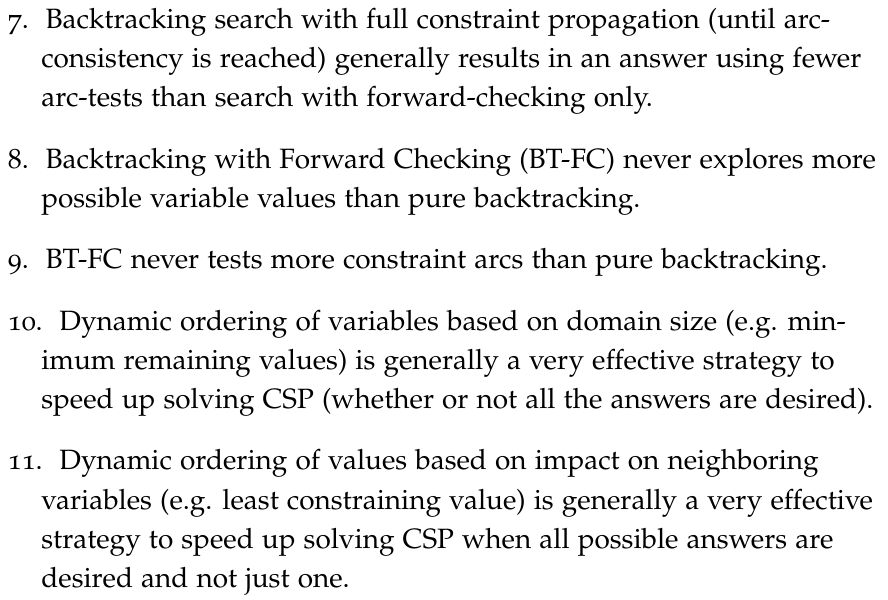
\includegraphics[width=\linewidth]{./assets/201807261947.png}
\end{figure}
\pagebreak
\begin{solution}{}~
\begin{enumerate}
\item True
\item False
\item True
\item True
\item False
\item False
\item True
\item True
\item True
\item False
\item True
\end{enumerate}
\end{solution}

% Question 5
\begin{figure}[h!]
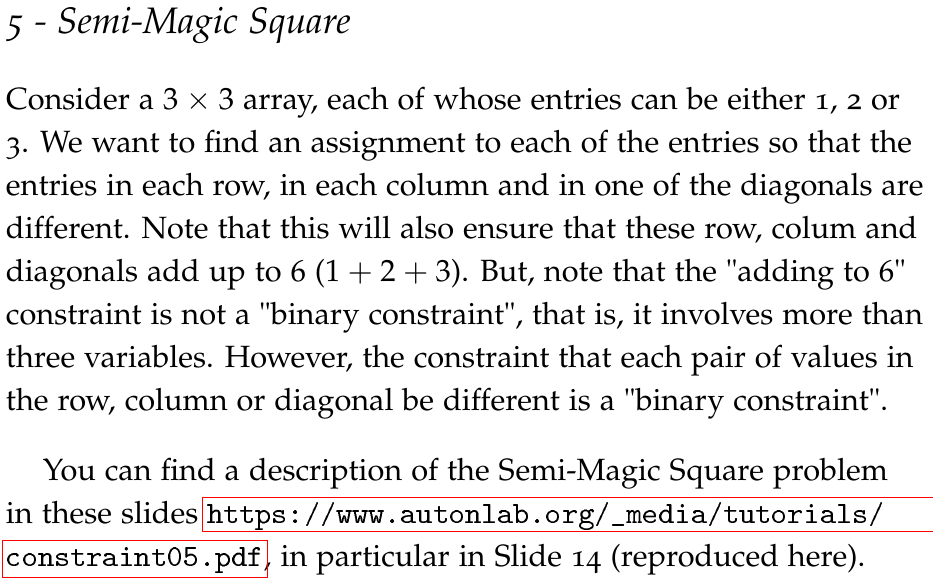
\includegraphics[width=\linewidth]{./assets/201807261948.png}
\end{figure}
\pagebreak
\begin{figure}[h!]
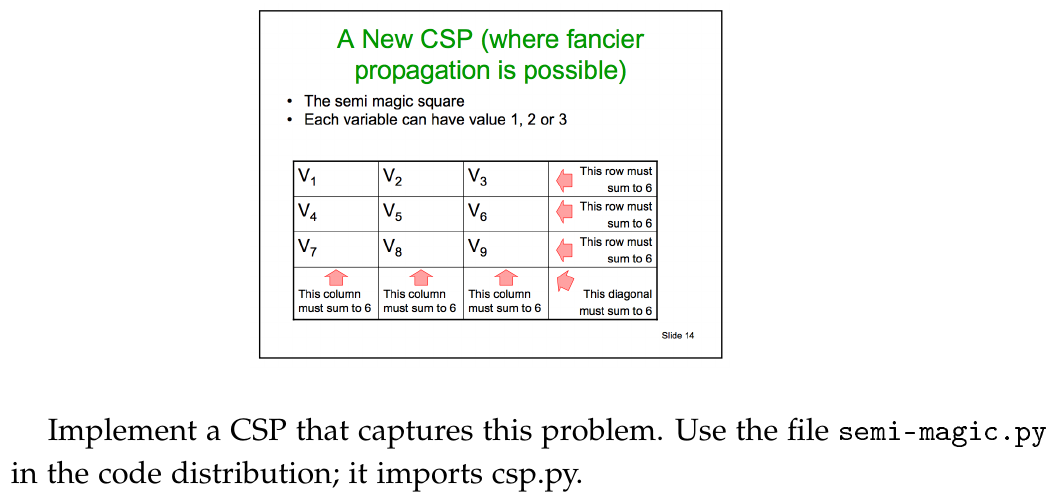
\includegraphics[width=\linewidth]{./assets/201807261949.png}
\end{figure}
\pagebreak
\begin{figure}[h!]
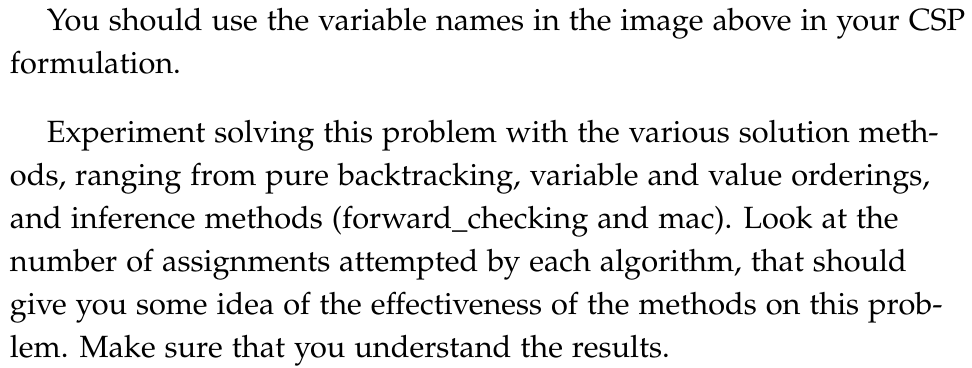
\includegraphics[width=\linewidth]{./assets/201807261950.png}
\end{figure}

\begin{solution}{}~\\

\lstinputlisting[language=Python]{semi-magic.py}

\textbf{Sequence produced: 123231312}
\end{solution}

% Question 6
\begin{figure}[h!]
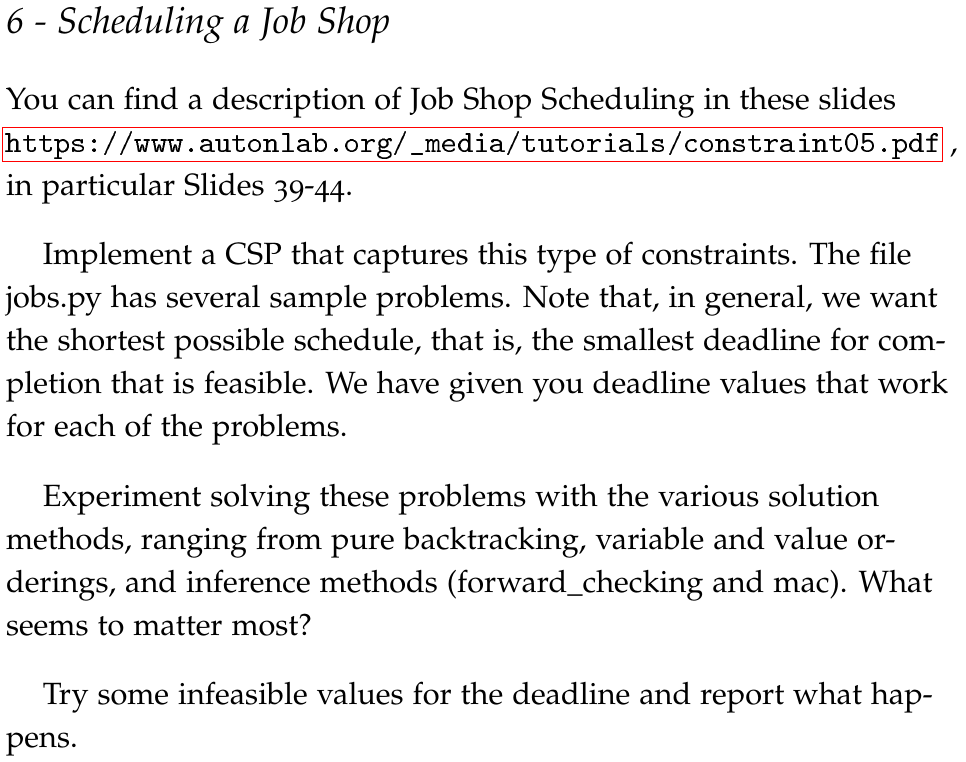
\includegraphics[width=\linewidth]{./assets/201807261951.png}
\end{figure}
\pagebreak
\begin{solution}{}~\\
\textbf{INCOMPLETE, TO BE COMPLETED.}
\end{solution}

%\lstinputlisting[language=Python]{pset5.py}

\end{document}
